\subsection{Reconstruction}

As the sample is rotated each detector pixel collects an intensity \(I(\theta) = I_{n}e^{-k(\theta)}\) at discrete (\(n\)) angles through a full rotation of the sample; where \(I_{n}\) is the unattenuated radiation intensity from the source to the detector, \(k\) is the attenuation caused by the sample along a detected ray an \(I(n)\) is the measured intensity, see \figurename~\ref{fig:OPT_digram}.
Rays from the sample to the detector approximate straight lines, and so the the rays reaching the detector with a line integrals.
A projection is then the resulting intensity profile at the detector for a rotation angle, and the integral transform that results in \(P_\theta(v)\)
% \(f(I_i,\theta_n) \)
is the \gls{Radon transform}.
% This is defined mathematically as:

\begin{align}
    \intertext{The equation of a set of parallel rays from a source passing through the specimen to a point \(v\) along the detector is:}
    &X\cos(\theta) + Y\sin(\theta) - v = 0 \\
    \intertext{Projecting many such rays through a sample with structure \(f(X,Y)\) gives:}
    P_\theta(v) = &\int_{\infty}^{\infty} \int_{\infty}^{\infty} f(X,Y)\delta (x\cos(\theta)+y \sin(\theta)-v)dX dY
\end{align}

% \begin{figure}
%     \centering
%     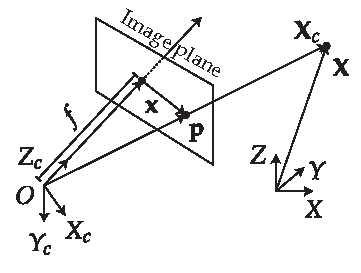
\includegraphics{coordinate_system}
%     \caption{Coordinate system}
%     \label{fig:coordinate_system_flopt}
% \end{figure}

Where \(P_\theta(v)\) is the \gls{Radon transform} of \(f(X,Y)\) which represents the contrast image of \gls{2D} slice of the specimen.
The \gls{Radon transform} of an image produces a \gls{sinugram} as in \figurename~\ref{fig:rawinputs}


% A parallel projection is then just the combination of line integrals  \(f(I) \) for a constant. % for a constant.

An inverse \gls{Radon transform} is used to recover the original object from the projection data; which is achieved by taking the \gls{Fourier transform} of each projection measurement, then reordering the information from the sample into the respective position in Fourier space.
This is valid due to the Fourier Slice theorem~\cite{bracewellStripIntegrationRadio1956} (see Appendix~\ref{appendix:fourierslice} for a derivation), which states that the \gls{Fourier transform} of a parallel projection is equivalent to a 2D slice of the Fourier transform of the original sample.
%A high pass filter such as a ramp filter is commonly used to counter the blurring caused by this oversampling.
% \gls{FBP} can be thought of as smearing the projection data across the image plane, and is expressed in equation form as:
\begin{align}
f_{\text{fpb}}(X,Y) = \int_{0}^{\pi} Q_\theta (X\cos(\theta)+Y\sin(\theta),\theta)dXdY
\end{align}

Where \(Q_\theta \) is the filtered projection data, and \(f_{\text{fpb}}(X,Y)\) is the back-projected image.
A spatial filtering step is applied during back-projection to avoid spatial frequency oversampling during the object’s rotation (see \figurename~\ref{fig:iradon_filter})
a high pass filter is commonly used to compensate for the perceived blurring.
The blurring arises as \(Q_\theta \) is back-projected (smeared) across the image plane for each angle of reconstruction; which means that not only does the back-projection contribute at the line it is intended to (along line \(C\) in \figurename~\ref{fig:coordinate_system_flopt}), but all other points along the back-projecting ray.
% The blurring occurs as \(Q_\theta\) makes the same contribution to the reconstruction for each angle
% will make the same contribution to the reconstruction at all of these points. Therefore, one could say that in the reconstruction process each filtered projection, Qe, is smeared back, or backprojected, over the image plane.
